% !TEX program = xelatex
% !TEX encoding = UTF-8
\documentclass[10pt,twocolumn]{article}

%% ========== Page Layout ==========
\usepackage[top=1.7cm, bottom=1.8cm, left=1.7cm, right=1.7cm, columnsep=0.7cm]{geometry}

%% ========== Fonts ==========
\usepackage{fontspec}
\setmainfont{Times New Roman}
\setsansfont{Arial}
\setmonofont{Courier New}

%% ========== Microtype & Justification (critical for English two-column) ==========
\usepackage{microtype}
\usepackage{ragged2e}
\setlength{\emergencystretch}{3em}
\hyphenpenalty=50

%% ========== Headers & Footers ==========
\usepackage{fancyhdr}
\pagestyle{fancy}
\fancyhf{}
\fancyhead[L]{\small\itshape AdaIN StyleKV: Training-Free Style Transfer with Self-Attention KV Fusion and Adaptive Normalization}
\fancyhead[R]{\small\thepage}
\fancyfoot{}
\renewcommand{\headrulewidth}{0.4pt}
\setlength{\headheight}{14pt}

%% ========== Spacing ==========
\setlength{\parindent}{1em}
\setlength{\parskip}{0pt}
\setlength{\abovedisplayskip}{5pt plus 2pt minus 2pt}
\setlength{\belowdisplayskip}{5pt plus 2pt minus 2pt}
\raggedbottom
\tolerance=2000
\emergencystretch=3em
\hyphenpenalty=1000
\renewcommand{\topfraction}{0.95}
\renewcommand{\bottomfraction}{0.95}
\renewcommand{\textfraction}{0.05}
\renewcommand{\floatpagefraction}{0.7}
\renewcommand{\dbltopfraction}{0.95}
\renewcommand{\dblfloatpagefraction}{0.7}
\setcounter{topnumber}{3}
\setcounter{dbltopnumber}{3}
\setcounter{totalnumber}{5}
\setlength{\floatsep}{4pt plus 1pt minus 1pt}
\setlength{\textfloatsep}{6pt plus 1pt minus 2pt}
\setlength{\intextsep}{5pt plus 1pt minus 2pt}
\setlength{\dblfloatsep}{4pt plus 1pt minus 1pt}
\setlength{\dbltextfloatsep}{6pt plus 1pt minus 2pt}

%% ========== Tables & Figures ==========
\usepackage{booktabs}
\usepackage{multirow}
\usepackage{array}
\usepackage{graphicx}
\usepackage{caption}
\usepackage{placeins}
\usepackage{stfloats}
\usepackage{float}
\captionsetup{labelsep=period, labelfont={small,bf}, textfont={small}}
\captionsetup[table]{skip=2pt}
\captionsetup[figure]{skip=2pt}
\renewcommand{\figurename}{Fig.}
\renewcommand{\tablename}{Table}

%% ========== Math & Symbols ==========
\usepackage{amsmath,amssymb}
\newcommand{\cmark}{$\checkmark$}
\newcommand{\xmark}{$\times$}

%% ========== Section Titles (CVPR-style) ==========
\usepackage{titlesec}
\titleformat{\section}{\normalfont\large\sffamily\bfseries}{\thesection.}{0.6em}{}
\titleformat{\subsection}{\normalfont\normalsize\sffamily\bfseries}{\thesubsection.}{0.6em}{}
\titleformat{\subsubsection}{\normalfont\normalsize\itshape}{\thesubsubsection}{0.6em}{}
\titlespacing*{\section}{0pt}{1.1em}{0.45em}
\titlespacing*{\subsection}{0pt}{0.85em}{0.35em}
\titlespacing*{\subsubsection}{0pt}{0.65em}{0.25em}

%% ========== Hyperlinks ==========
\usepackage[hidelinks]{hyperref}

%% ========== Title Formatting ==========
\usepackage{titling}
\setlength{\droptitle}{-2.6cm}

\graphicspath{{figures/}}

\begin{document}

% ===== Title block + teaser + abstract (CVPR-style, spanning full width) =====
\twocolumn[{%
\begin{center}
  {\sffamily\bfseries\LARGE AdaIN StyleKV: Training-Free Style Transfer with Self-Attention\\[1pt]KV Fusion and Adaptive Instance Normalization for Diffusion Models}\\[4pt]
  {\large Junji Jiang \quad Zhuoliang Lv \quad Peiwen Yang}\\[1pt]
  {\large School of Computer Science and Engineering (Cyberspace Security),\\University of Electronic Science and Technology of China}\\[1pt]
  {\ttfamily \{junji.jiang, zhuoliang.lv, peiwen.yang\}@uestc.edu.cn}\\[4pt]
\end{center}

\begin{center}
  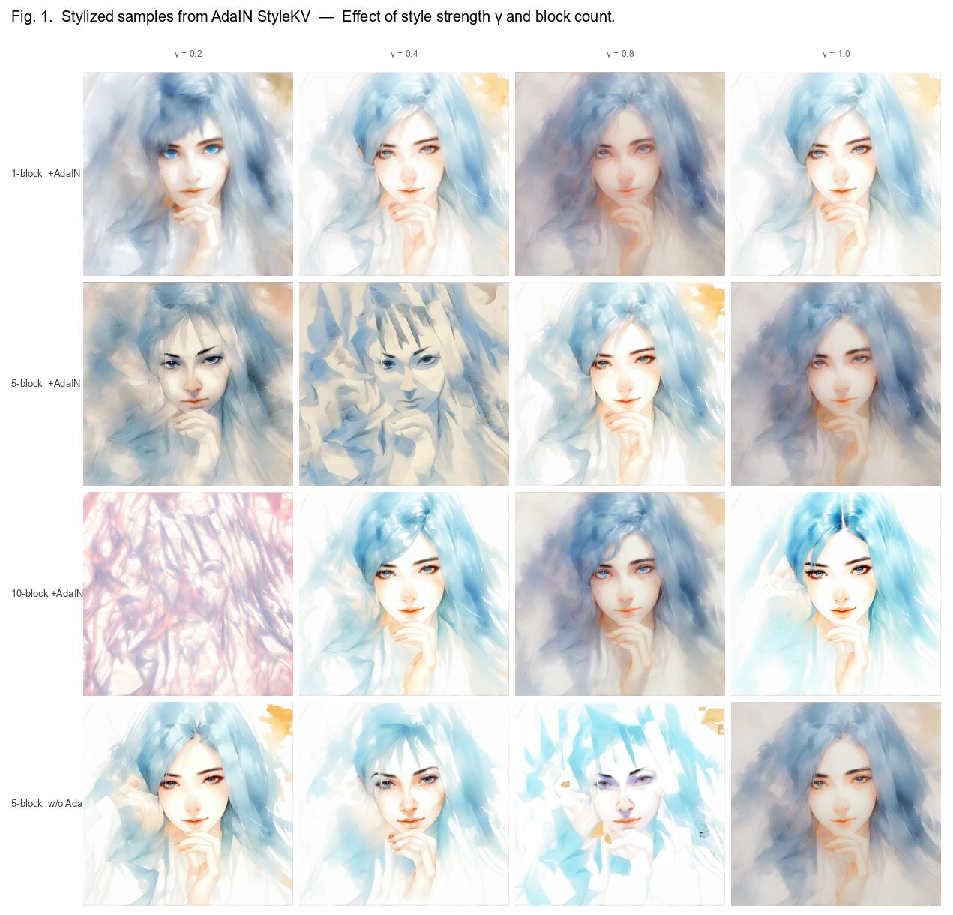
\includegraphics[width=0.50\textwidth]{fig_gallery.pdf}
  \captionof{figure}{Stylization results of AdaIN StyleKV. Horizontally, $\gamma$ increases from 0.2 to 1.0; vertically, 1-proc, 5-proc, and 10-proc configurations are shown with and without AdaIN. The 5-proc + AdaIN configuration (our full method) achieves a favorable balance between style intensity and content fidelity near $\gamma=0.6$.}
  \label{fig:gallery}
\end{center}

\vspace{0pt}
\begin{minipage}{\textwidth}
\begin{center}{\sffamily\bfseries\large Abstract}\end{center}
{\noindent Artistic style transfer seeks to impose the visual appearance of a reference image onto a content image without corrupting the latter's semantic structure. Diffusion models have pushed this task forward, but the solution landscape is split. Methods like InST and StyleDiffusion deliver convincing stylization through per-image optimization or inversion; training-free alternatives dispense with tuning, yet often stumble on structure preservation, color fidelity, or the absence of a straightforward intensity control. We introduce AdaIN StyleKV, a framework that keeps the SDXL backbone frozen and layers on three training-free mechanisms. A Canny ControlNet supplies explicit edge-map conditioning to anchor spatial layout. Inside UNet block \texttt{up\_blocks.0.attentions.1}, a selective KV fusion module---inspired by Style Injection---caches key--value features from the style image at a small subset of self-attention processors and mixes them with content KV through a single scalar $\gamma$, with no gradient steps involved. At the same target block, a cross-modal AdaIN module, adapted from StyleStudio [31], uses channel-wise statistics of a pretrained image embedding to pull text-condition features toward the style reference's color distribution. Across 5000 MS COCO $\times$ WikiArt pairs and seven variant configurations, the 5-processor StyleKV setup without AdaIN reaches the lowest Art-FID (85.43), while enabling AdaIN brings LPIPS from 0.629 down to 0.599 at a modest Art-FID trade-off (90.76). We also release StyleKV Control Studio, a Gradio frontend for real-time manipulation of $\gamma$, Canny thresholds, and AdaIN coefficients.}

\end{minipage}
\vspace{6pt}
}]

\vspace{-4pt}
\noindent{\small\textbf{Keywords:} style transfer; diffusion models; self-attention; adaptive instance normalization; training-free; ControlNet}
\vspace{6pt}

%% ================================================
%% 1. Introduction
%% ================================================
\section{Introduction}

Artistic style transfer has been an active research area in computer vision for over two decades. Given a content image and a style reference, the objective is to synthesize an output that preserves the semantic structure and spatial layout of the former while adopting the texture, brushwork, and color palette of the latter.

Early approaches tackled the problem through non-parametric texture synthesis [1] and optimization over VGG Gram matrices [2]. Feedforward networks [3,4] and Adaptive Instance Normalization (AdaIN) [4] subsequently brought real-time performance. Generative adversarial networks further improved output fidelity [5,6,7]. Despite this steady progress, each paradigm left unresolved tensions. GAN-based methods generalize poorly beyond style domains observed during training. Optimization-based formulations remain computationally expensive. And across these early families, no mechanism emerged for continuously trading off style intensity against content preservation.

Diffusion models reshaped the generative landscape [8,9,10]. Stable Diffusion [11] in particular, by working in a compressed latent space and conditioning on text via cross-attention, made high-resolution synthesis practical. Researchers adapted this machinery to style transfer almost immediately [12,13,14,15,16,17]. Yet a cluster of difficulties has proven stubborn. InST [12] and StyleDiffusion [13] produce strong results, but every new style image triggers its own round of gradient updates or textual inversion; the per-style cost adds up quickly outside small-scale settings. Training-free methods such as DiffStyle [14] and Style Injection [16] avoid optimization altogether, only to run into a different set of problems—content layout can drift, and global color often gets lost because self-attention, for all its sensitivity to local texture, carries no notion of an overall palette. Equally limiting, hardly any of these methods expose a clean, continuous parameter for dialing style intensity up and down.

These observations motivate AdaIN StyleKV, a framework that combines three lightweight, training-free interventions within a frozen SDXL model. The design emerged incrementally. An initial prototype applied AdaIN on one or two UNet target blocks---selected following InstantStyle's [17] guidance on block importance---to align text and image conditions. Color coordination improved, but brushstroke and texture patterns remained largely unchanged. This finding led to the incorporation of a KV fusion mechanism inspired by Style Injection [16]: rather than a wholesale replacement of key--value features, the framework caches style-image K/V from a small set of self-attention processors within \texttt{up\_blocks.0.attentions.1} and blends them with content K/V via a single coefficient $\gamma \in [0,1]$. The fusion is confined to this single block rather than broadcast across the UNet, limiting computational overhead.

The second mechanism addresses what KV fusion alone misses. Drawing on the cross-modal AdaIN formulation from StyleStudio [31], a pretrained image encoder (IP-Adapter's, in the implementation) extracts a style embedding whose channel-wise statistics are used to re-normalize text-condition features at the same target block. The operation preserves the semantic content of the text embedding while shifting its color distribution toward the style reference. Together with Canny ControlNet, which supplies an explicit edge-map scaffold to anchor spatial structure, the three components---structure, texture, and color---constitute the complete pipeline.

Experiments span 5000 COCO [18] $\times$ WikiArt [19] pairs evaluated across seven variant configurations under three metrics: Art-FID [20] (style-domain proximity), FID [21] (content-domain proximity), and LPIPS [22] (per-pair perceptual distance). The 5-processor StyleKV configuration without AdaIN achieves the lowest Art-FID in the sweep (85.43), though LPIPS rises to 0.629. Enabling AdaIN raises Art-FID to 90.76 but reduces LPIPS to 0.599, indicating that AdaIN moderates aggressive texture transfer in favor of perceptual coherence. Beyond aggregate metrics, the experiments dissect the influence of block count, processor count, $\gamma$, and the AdaIN toggle on stylization behavior. A Gradio-based interface, StyleKV Control Studio, accompanies the method and supports real-time parameter adjustment with live Canny preview.

%% ================================================
%% 2. Related Work
%% ================================================
\section{Related Work}

\subsection{Neural Style Transfer}

Gatys et al. [2] established the neural style transfer paradigm by matching Gram matrices of VGG [23] features within an iterative optimization. The push toward real-time performance that followed produced several influential designs. Johnson et al. [24] trained feedforward transformation networks with perceptual losses. Huang \& Belongie [4] introduced AdaIN, aligning channel-wise statistics to enable arbitrary style transfer in a single forward pass. Attention-based mechanisms [25], Transformer architectures [26], reversible flows [27], and dual-branch learning frameworks [28] each contributed further refinements. Relative to Gatys' original optimizer, speed and generalization improved markedly; the remaining difficulty is that heavily abstract or non-photorealistic styles tend to expose the limits of VGG-centric feature matching, which can smear fine detail and flatten subtle texture variations.

\subsection{GAN-Based Style Transfer}

In the GAN era, CycleGAN [5] demonstrated that cycle-consistency losses could steer unpaired image translation; StarGAN [6] extended the principle to multi-domain translation within a single model. StyleGAN [7] and its successors [29,30] brought remarkably fine-grained latent-space control. It is worth noting, however, that StyleGAN functions as an unconditional generator, not a cross-domain translator. Repurposing it for arbitrary style transfer demands additional fine-tuning or disentanglement procedures, and generalization beyond the training distribution remains fragile.

\subsection{Diffusion-Based Style Transfer}

Diffusion models have become the dominant paradigm for high-quality image generation. Among them, latent diffusion models (LDM) [11] achieve efficient training and inference by compressing images into a low-dimensional latent space. For style transfer tasks, researchers have proposed various diffusion-based methods:

InST [12] embeds style images into the text token space via inversion. The stylization quality is strong, but each new reference demands its own optimization run. StyleDiffusion [13] introduces CLIP-based losses alongside fine-tuning to disentangle content and style in feature space---again, a per-image procedure. DiffStyle [14] sidesteps training by operating in the diffusion H-space, though applying it directly to Stable Diffusion can perturb semantic layout. Style Injection [16] overwrites the K and V within self-attention layers using style-image features. The approach is training-free and preserves a reasonable degree of structure, but absent an explicit spatial constraint, content geometry can still drift. InstantStyle [17] contributed the important empirical finding that not all UNet blocks are equally style-sensitive; concentrating injection on a carefully chosen subset is both cheaper and more effective than broadcasting uniformly. StyleStudio [31] further explored selective gating of style elements under text-prompt guidance.

\begin{table}[htbp]
  \centering
  \caption{Comparison of our method with representative style transfer methods. TF: Training-Free (no fine-tuning); SP: Structure Preservation (explicit spatial constraints); CT: Color Transfer (global color handling); CI: Controllable Intensity (explicit continuous control).}
  \label{tab:method_comparison}
  \small
  \setlength{\tabcolsep}{3pt}
  \begin{tabular}{lcccc}
    \toprule
    Method & TF & SP & CT & CI \\
    \midrule
    InST [12] & \xmark & \xmark & \cmark & \xmark \\
    StyleDiffusion [13] & \xmark & \xmark & \cmark & \cmark \\
    DiffStyle [14] & \cmark & \xmark & \xmark & \xmark \\
    Style Injection [16] & \cmark & \xmark & \xmark & \xmark \\
    InstantStyle [17] & \cmark & \xmark & \xmark & \xmark \\
    \textbf{AdaIN StyleKV (Ours)} & \cmark & \cmark & \cmark & \cmark \\
    \bottomrule
  \end{tabular}
\end{table}

Table~\ref{tab:method_comparison} situates AdaIN StyleKV relative to these baselines. The distinguishing combination is training-free operation paired with explicit Canny edge conditioning for structure, a dedicated cross-modal AdaIN path for global color, and a single scalar $\gamma$ that provides continuous intensity control.

\subsection{Conditional Control in Diffusion Models}

ControlNet [15] introduced zero-convolution layers to attach spatial conditions (edges, depth, pose) to a frozen diffusion model without degrading its pretrained weights. We use the Canny variant: an edge map extracted from the content image is fed through a trainable copy of the UNet encoder, whose outputs are injected into the skip connections and middle block of the frozen decoder. All experiments use SDXL with the matching ControlNet weights \texttt{diffusers/controlnet-canny-sdxl-1.0}. SDXL was chosen for its higher native resolution and richer semantic representations.

%% ================================================
%% 3. Method
%% ================================================
\section{Method}

AdaIN StyleKV operates on a frozen SDXL backbone with a Canny ControlNet attached. Inference proceeds through five stages, within which three lightweight mechanisms are interleaved: cross-modal AdaIN for color alignment, selective KV fusion for texture transfer, and Canny edge conditioning for spatial anchoring.

\subsection{Overall Framework}

\medskip
\noindent{\bfseries Stage 1: Preprocessing.} The VAE encoder maps content and style images to latents $z_{\text{content}}$ and $z_{\text{style}}$. A Canny edge detector (with adjustable thresholds, exposed in the frontend) extracts a contour map from the content image, producing the spatial condition $c_{\text{canny}}$ for ControlNet.

\medskip
\noindent{\bfseries Stage 2: DDIM Inversion.} DDIM inversion is applied to both latents independently, yielding noise trajectories $\{z_t^{\text{content}}\}$ and $\{z_t^{\text{style}}\}$ spanning all $T$ timesteps. These trajectories serve as the temporal backbone for both AdaIN modulation and KV caching: at each $t$, the style latent supplies K/V features while the content latent undergoes the actual denoising.

\medskip
\noindent{\bfseries Stage 3: Cross-Modal AdaIN.} At each denoising timestep, before the UNet forward pass, text-condition embeddings at the target block(s) are intercepted and re-normalized via AdaIN using channel statistics from a pretrained image embedding of the style image (IP-Adapter's encoder, in our setup). The mean and variance of the already-computed text features are shifted toward the style embedding's distribution; no additional adapters are trained.

\medskip
\noindent{\bfseries Stage 4: KV Fusion.} We fix the injection site at UNet block \texttt{up\_blocks.0.attentions.1}. At each timestep $t$, during the style latent's forward pass we cache $\{K_{\text{style}}, V_{\text{style}}\}$ from a selected subset of self-attention processors within this block. During the content latent's denoising step at the same $t$, the cached features are blended with content K/V via:
\[
\begin{aligned}
K_{\text{fused}} &= (1-\gamma)K_{\text{content}} + \gamma K_{\text{style}},\\
V_{\text{fused}} &= (1-\gamma)V_{\text{content}} + \gamma V_{\text{style}},
\end{aligned}
\quad \gamma \in [0,1].
\]
Non-target processors run standard self-attention; the content query $Q_{\text{content}}$ is never modified.

\medskip
\noindent{\bfseries Stage 5: Decoding.} After $T$ denoising steps, the final latent $z_0$ is passed through the VAE decoder to produce the stylized output.

\begin{figure}[htbp]
  \centering
  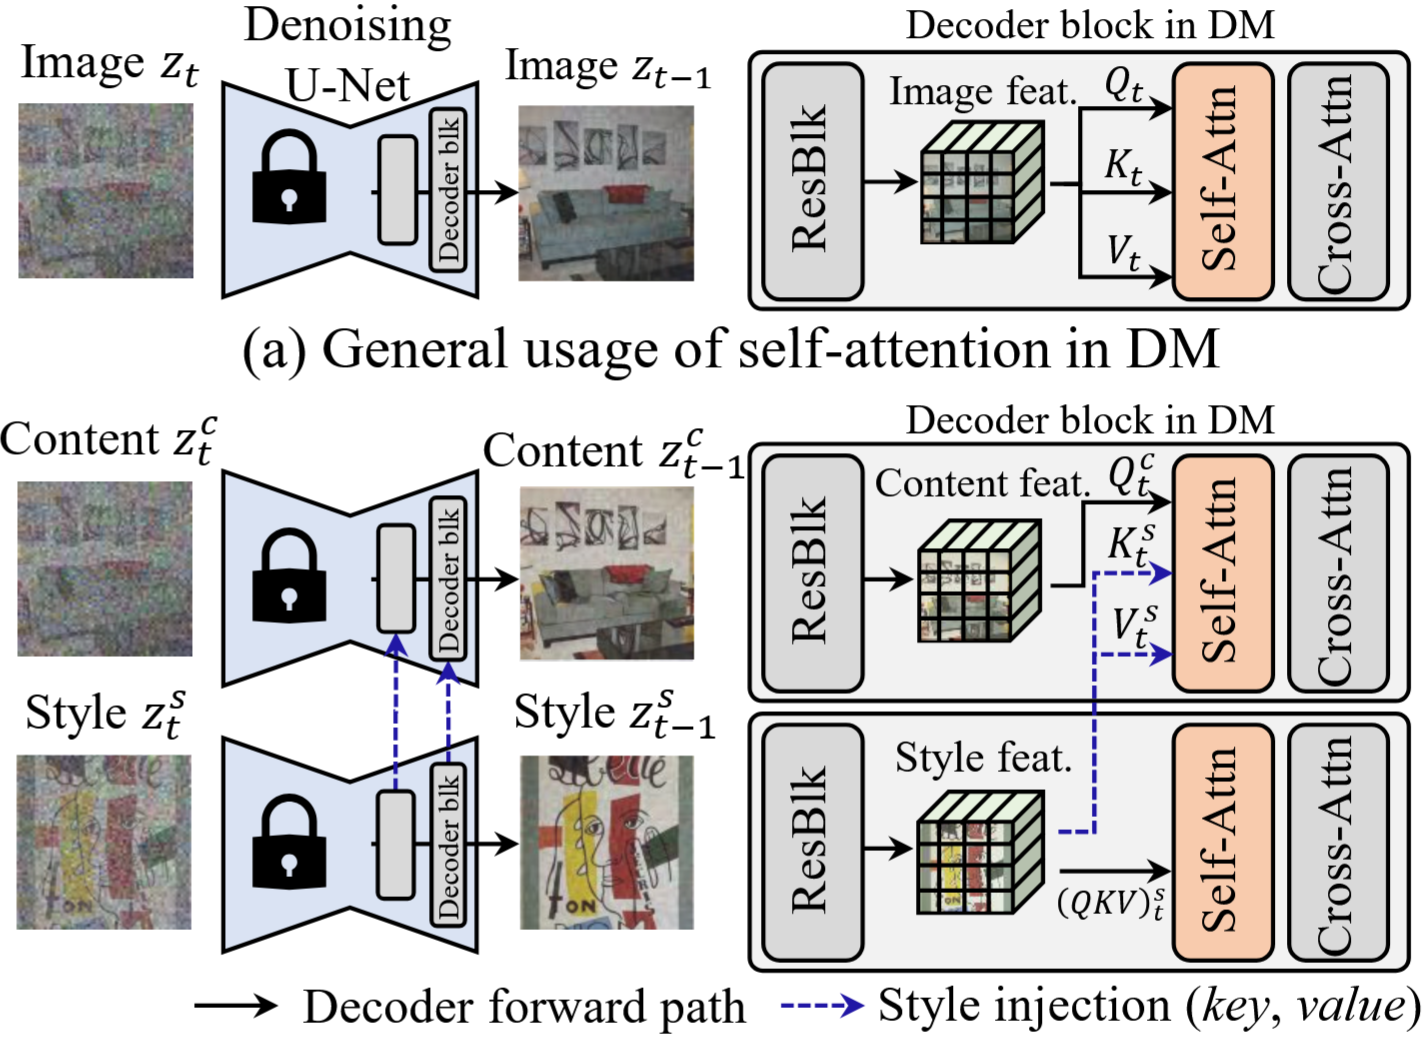
\includegraphics[width=\columnwidth]{Snipaste_2026-06-12_21-47-51.png}
  \caption{Overall pipeline of AdaIN StyleKV. Content and style images enter the VAE in parallel; a Canny edge map of the content anchors ControlNet. DDIM inversion produces latent trajectories for both images. Cross-modal AdaIN fuses text and image conditions at the target UNet block, and cached style K/V are blended with content K/V inside selected self-attention processors. The VAE decoder produces the final output.}
  \label{fig:pipeline}
\end{figure}

Fig.~\ref{fig:pipeline} gives the visual summary of this five-stage flow.

\subsection{Selective KV Fusion}

\subsubsection{Self-Attention Recap}

The UNet self-attention layer projects a feature map $X$ into query, key, and value:
\begin{equation}
Q = X W_Q, \quad K = X W_K, \quad V = X W_V \label{eq:qkv}
\end{equation}
then computes:
\begin{equation}
\text{Attention}(Q, K, V) = \text{softmax}\!\left(\frac{QK^T}{\sqrt{d_k}}\right)V \label{eq:attention}
\end{equation}
In standard generation, $Q$, $K$, and $V$ are all projected from the same feature map. For style transfer, the key insight is to retain $Q$ from the content image---it encodes spatial organization---while blending content $K,V$ with those from the style image, which carry texture, brushstroke, and palette information. The resulting attention map retrieves style patterns and places them at the appropriate content locations.

\begin{figure}[htbp]
  \centering
  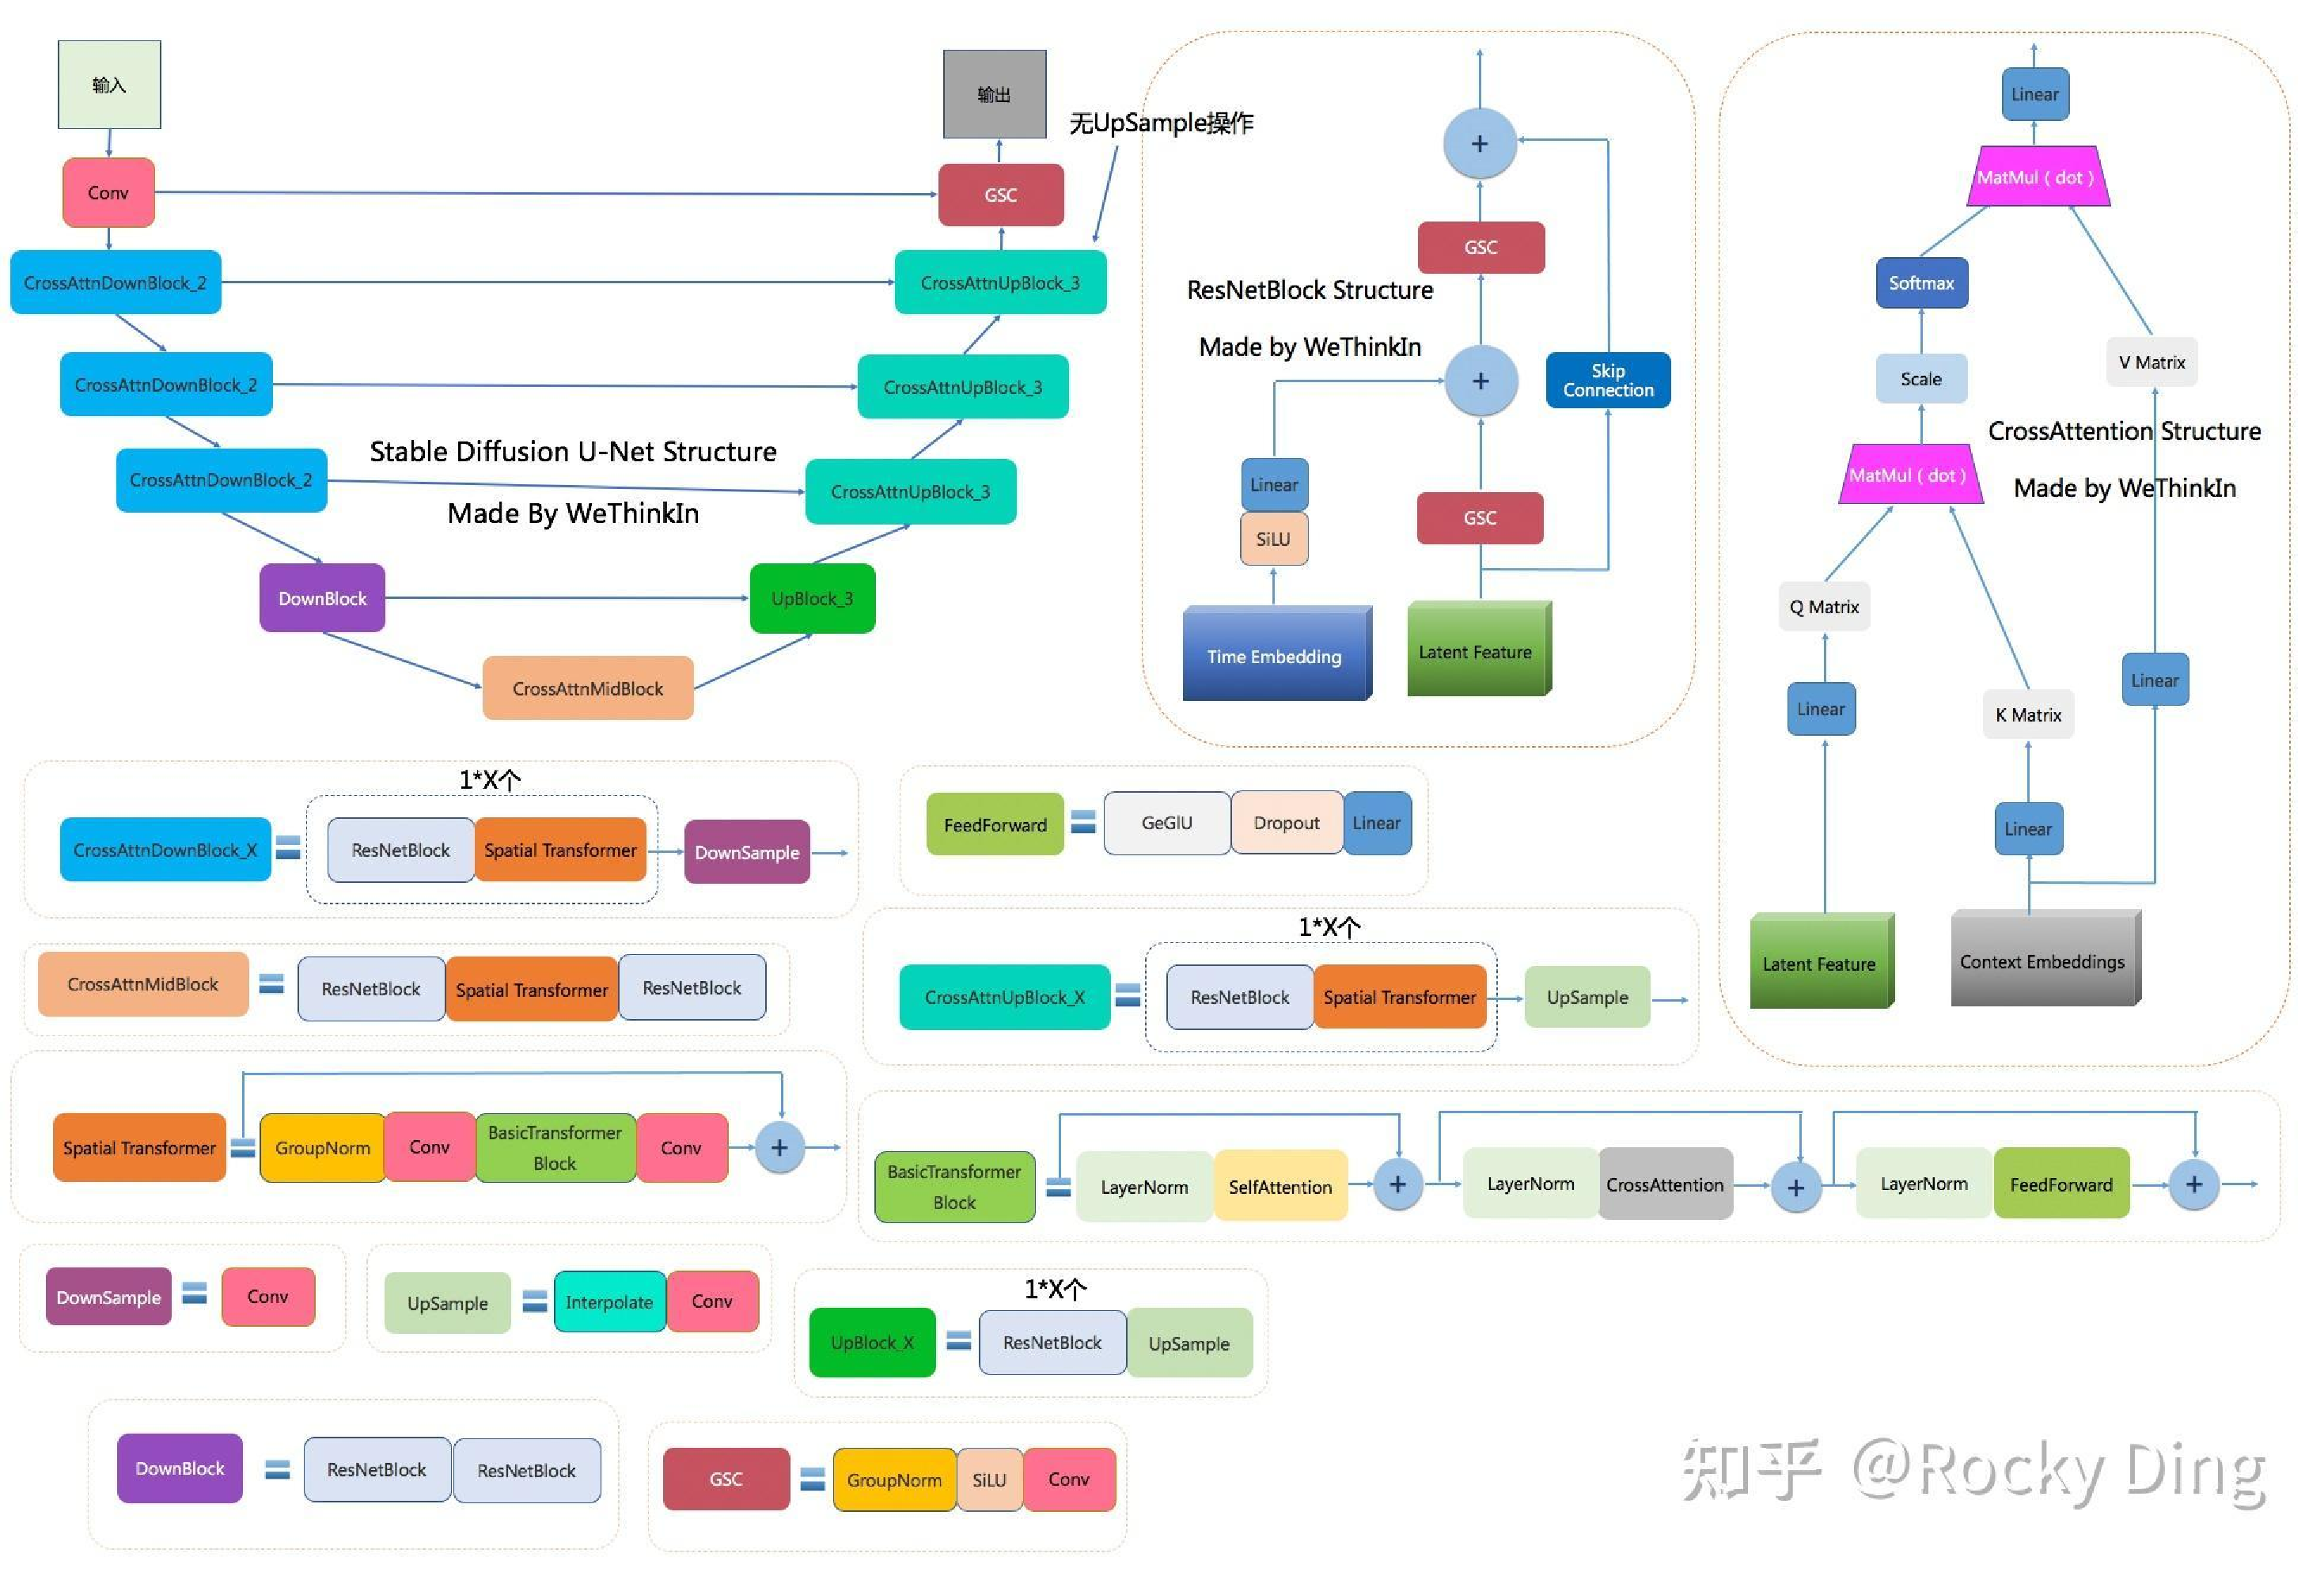
\includegraphics[width=\columnwidth]{fig_unet_arch.pdf}
  \caption{U-Net architecture in Stable Diffusion, showing the encoder, middle block, and decoder with their ResNet and self-attention layers. We confine KV fusion to the target block \texttt{up\_blocks.0.attentions.1} (red), leaving all other attention processors untouched.}
  \label{fig:unet_arch}
\end{figure}

Fig.~\ref{fig:unet_arch} shows the UNet layout and highlights \texttt{up\_blocks.0.attentions.1}, the sole injection site for all StyleKV experiments.

\subsubsection{Weighted KV Fusion}

Following Style Injection [16], the self-attention processors inside \texttt{up\_blocks.0.attentions.1} are targeted for KV fusion. Rather than overwriting features, the method blends content and style representations linearly:
\begin{equation}
K_{\text{fused}} = (1 - \gamma) K_{\text{content}} + \gamma K_{\text{style}} \label{eq:kfusion}
\end{equation}
\begin{equation}
V_{\text{fused}} = (1 - \gamma) V_{\text{content}} + \gamma V_{\text{style}} \label{eq:vfusion}
\end{equation}
with $\gamma \in [0, 1]$. The coefficient functions as a continuous control: $\gamma{=}0$ leaves content K/V intact, $\gamma{=}1$ uses pure style K/V, and intermediate values interpolate smoothly. The operation incurs no gradient overhead---two vector additions and one scalar multiplication per processor---and in early experiments, linear blending produced fewer abrupt artifacts than hard KV replacement.

\subsubsection{Which Block, Which Processors?}

InstantStyle [17] demonstrated empirically that not all UNet blocks contribute equally to style transfer. Building on this finding, we confine injection to a single decoder block, \texttt{up\_blocks.0.attentions.1}. All experiments labeled ``StyleKV'' in this paper operate exclusively at this site. Within the block, the number of self-attention processors participating in KV fusion is varied:

\begin{itemize}
  \setlength{\itemsep}{0pt}
\item {\bfseries 1 proc}: minimal injection, mostly content
\item {\bfseries 5 procs} (our default): the sweet spot in our experiments
\item {\bfseries 10 procs}: heavier injection, stronger style but can eat into fine detail
\end{itemize}

Five processors yielded the most even trade-off between style transfer and content preservation; this configuration is therefore used as the default throughout the paper and in the frontend unless stated otherwise.

\begin{table}[htbp]
  \centering
  \caption{Target block configurations in the early naive AdaIN prototype. \texttt{1blk}/\texttt{2blk} indicate the number of UNet target blocks where AdaIN is applied; in contrast, StyleKV experiments are fixed at \texttt{up\_blocks.0.attentions.1} and vary the number of self-attention processors.}
  \label{tab:adain_target_blocks}
  \footnotesize
  \setlength{\tabcolsep}{3pt}
  \begin{tabular}{p{1.5cm}p{3.6cm}p{2.5cm}}
    \toprule
    Config & AdaIN Target UNet Block(s) & Variant \\
    \midrule
    1blk & \texttt{up0.attn1} & V1: \texttt{adain\_1blk} \\
    2blk & \texttt{up0.attn1}; \texttt{down2.attn1} & V2: \texttt{adain\_2blk} \\
    \bottomrule
  \end{tabular}
\end{table}

\subsection{Cross-Modal AdaIN for Text and Image Conditions}

KV fusion handles texture effectively, but color transfer poses a distinct challenge. Blending K/V pairs captures local brushwork well yet often misses the global palette, producing the right textures in the wrong colors. The StyleStudio [31] paper pointed out that AdaIN across text and image modalities can close this gap, and we adapt that insight directly into our pipeline.

A frozen image encoder (the one provided with IP-Adapter, in our implementation) produces a style embedding $f_{\text{style}}$. At the same target UNet block where KV fusion happens, we grab the text-condition features $f_{\text{text}}$ that are already in the pipeline and re-normalize them:
\begin{equation}
f_{\text{adain}} = \sigma(f_{\text{style}}) \left( \frac{f_{\text{text}} - \mu(f_{\text{text}})}{\sigma(f_{\text{text}})} \right) + \mu(f_{\text{style}}) \label{eq:adain}
\end{equation}
with $\mu(\cdot)$, $\sigma(\cdot)$ computed per channel. In code we expose two extra knobs, $\alpha$ and $\beta$:
\begin{equation}
f_{\text{adain}}^{(\beta)} = \sigma(f_{\text{style}}) \left( \frac{f_{\text{text}} - \mu(f_{\text{text}})}{\sigma(f_{\text{text}})} \right) + \beta \mu(f_{\text{style}})
\end{equation}
\begin{equation}
f_{\text{out}} = (1-\alpha) f_{\text{text}} + \alpha f_{\text{adain}}^{(\beta)}.
\end{equation}
At $\alpha{=}1.0$, $\beta{=}1.0$ (our defaults) this collapses to Eq.~\ref{eq:adain}. Internally, the text embedding's semantic direction remains intact while its channel-wise statistics are aligned with the style reference. The diffusion model thus receives the same content guidance but with color statistics drawn from the style image. No additional training or adapter modules are required---only a mean-and-variance shift applied at the appropriate point in the network.

\subsection{ControlNet Integration}

Canny ControlNet gives us a spatial scaffold. It takes the content image's edge map, pushes it through a trainable copy of the UNet encoder (frozen at initialization via zero-convolutions), and injects the outputs into the frozen decoder's skip connections and middle block. We use the SDXL-matched weights \texttt{diffusers/controlnet-canny-sdxl-1.0} as-is, with no further training.

\subsection{Inference}

Everything above happens at inference time inside a completely frozen $\epsilon_\theta$. At timestep $t$, with text prompt $c$ and Canny condition $c_{\text{canny}}$, the noise prediction is:
\begin{equation}
\hat{\epsilon} = \epsilon_\theta(z_t, t, c, c_{\text{canny}}) \label{eq:inference}
\end{equation}
The AdaIN modulation and KV fusion are injected as side-effects during the forward pass through the target block; the model weights never move. The output follows the five-stage pipeline described earlier.

%% ================================================
%% 4. Experiments and Results
%% ================================================
\section{Experiments and Results}

\begin{figure*}[!b]
  \centering
  
\includegraphics[width=\textwidth]{image2.pdf}
  \caption{Quantitative comparison of 7 method variants across FID, Art-FID, and LPIPS metrics (lower is better for all three). FID reflects distribution distance from the content domain, Art-FID reflects proximity to the target artistic style domain, and LPIPS reflects the perceptual-level image change magnitude. V6 (Ours w/o AdaIN) achieves the lowest Art-FID, indicating stronger style injection; compared with V6, the full method V7 (Ours AdaIN, $\gamma=0.6$) reduces LPIPS, indicating milder perceptual change.}
  \label{fig:variants2}
\end{figure*}

\subsection{Experimental Setup}

\subsubsection{Datasets}

{\bfseries Content dataset:} We use 5000 content images from the MS COCO 2017 dataset [18], each accompanied by a corresponding text prompt to assist the diffusion model in understanding the image content.

{\bfseries Style dataset:} We use 5000 style images from the WikiArt dataset [19], covering various artistic styles such as Impressionism, Cubism, and Abstract art.

{\bfseries Image pairing:} 5000 content images and 5000 style images are paired one-to-one in sequential order, yielding 5000 pairs in total.

{\bfseries Data scale:} A total of 5000 stylized images are generated for quantitative evaluation.

\subsubsection{Evaluation Metrics}

We track three numbers, all in the lower-is-better direction, but they capture different things. {\bfseries Art-FID} [20] measures distributional distance from the target style set---our primary gauge of how well the style came through. {\bfseries FID} [21] does the same against the content set, giving a rough proxy for content-domain proximity (though it's too global to serve as a standalone structure-preservation score). {\bfseries LPIPS} [22] computes per-pair perceptual distance between each output and its content image. A low LPIPS means the image ``reads'' similar to the original; a high LPIPS means the transfer visibly shifted things. Since any interesting stylization will push LPIPS up somewhat, we read it alongside Art-FID and FID, not in isolation. No single metric tells the full story here---the three-way trade-off is the point.

\subsubsection{Hardware Configuration and Hyperparameters}

Experiments were conducted on the AutoDL platform using a rented NVIDIA V100-32GB GPU. Hardware and hyperparameter configurations are shown in Table~\ref{tab:hardware} and Table~\ref{tab:hyperparams}, respectively.

\begin{table}[htbp]
  \centering
  \caption{Hardware configuration and environment.}
  \label{tab:hardware}
  \small
  \begin{tabular}{ll}
    \toprule
    Configuration Item & Parameter \\
    \midrule
    GPU & NVIDIA V100 32GB $\times$ 1 \\
    Acceleration Library & xformers \\
    Sampling Steps & 30 steps (DDIM) \\
    Resolution & 512$\times$512 (center crop) \\
    Total Generated Images & 5000 \\
    \bottomrule
  \end{tabular}
\end{table}

\begin{table}[htbp]
  \centering
  \caption{Hyperparameter settings. $\gamma=0.6$ is the experimentally determined favorable trade-off point (see Section~4.4 for sensitivity analysis); KV fusion defaults to 5 self-attention processors in \texttt{up\_blocks.0.attentions.1}; AdaIN fusion intensity defaults to 1.0.}
  \label{tab:hyperparams}
  \small
  \begin{tabular}{lll}
    \toprule
    Parameter & Value & Description \\
    \midrule
    $\gamma$ & 0.6 & Style fusion intensity \\
    \texttt{up0.attn1} procs & 5 & KV fusion processor count \\
    adain\_alpha & 1.0 & AdaIN fusion intensity \\
    adain\_beta  & 1.0 & AdaIN fusion bias \\
    CFG scale & 6.0 & Classifier-free guidance \\
    DDIM steps & 30 & Diffusion sampling steps \\
    \bottomrule
  \end{tabular}
\end{table}

\subsection{Method Variant Design}

We evaluate seven configurations (Table~\ref{tab:variants}) that isolate different pieces of the pipeline. V1--V5 correspond to the early AdaIN-only prototype: V1/V2 turn AdaIN on at 1 or 2 target blocks, V3/V4 turn it off (same block counts), and V5 removes ControlNet while keeping AdaIN. V6 and V7 add 5-processor StyleKV fusion on top; V6 keeps AdaIN off, V7 is the full stack. A quick note on terminology: we reserve ``ablation'' for single-factor comparisons---V6 vs.\ V7 isolates AdaIN's effect, V1 vs.\ V5 isolates ControlNet. The 1blk/2blk and 1/5/10-proc variations are configuration sweeps and sensitivity analyses, not ablations in the strict sense.

\begin{table}[htbp]
  \centering
  \caption{Design of 7 method variants. CtrlN = ControlNet; Scope = target blocks (blk) or processors (p); KV = KV fusion enabled.}
  \label{tab:variants}
  \footnotesize
  \setlength{\tabcolsep}{2pt}
  \begin{tabular}{clccccc}
    \toprule
    \# & Variant & CtrlN & Scope & AdaIN & $\gamma$ & KV \\
    \midrule
    V1 & adain\_1blk       & \cmark & 1blk & \cmark & -- & \xmark \\
    V2 & adain\_2blk       & \cmark & 2blk & \cmark & -- & \xmark \\
    V3 & noadain\_1blk     & \cmark & 1blk & \xmark & -- & \xmark \\
    V4 & noadain\_2blk     & \cmark & 2blk & \xmark & -- & \xmark \\
    V5 & adain\_no\_ctrl    & \xmark & 1blk & \cmark & -- & \xmark \\
    V6 & proc05\_no\_adain  & \cmark & 5p & \xmark & 0.6 & \cmark \\
    V7 & proc05\_adain      & \cmark & 5p & \cmark & 0.6 & \cmark \\
    \bottomrule
  \end{tabular}
\end{table}

Fig.~\ref{fig:variant_progress} and Fig.~\ref{fig:variant_compare} present visual comparisons across different content--style pairings for intuitive observation of the differences among variants in style injection intensity, color coordination, and content preservation.

\begin{figure}[H]
  \centering
  
\includegraphics[width=\columnwidth]{fig_variant_progress.pdf}
  \caption{Horizontal comparison of outputs from different method configurations on the ``man'' content image. The upper labels indicate the corresponding method configuration, enabling intuitive comparison of each configuration's effect on style injection intensity and content preservation.}
  \label{fig:variant_progress}
\end{figure}

\begin{figure}[H]
  \centering
  
\includegraphics[width=\columnwidth]{fig_variant_compare.pdf}
  \caption{Method variant comparison on two different content--style pairings.}
  \label{fig:variant_compare}
\end{figure}

\FloatBarrier
\setcounter{figure}{6}

\subsection{Quantitative Results}

Table~\ref{tab:quant_results} and Fig.~\ref{fig:variants2} present the quantitative evaluation results of the 7 variants on 5000 generated images.

\begin{table}[htbp]
  \centering
  \caption{Quantitative evaluation results of 7 variants on 5000 generated images. FID measures distribution distance from the content domain (lower indicates closer overall feature distribution to original content); Art-FID measures distribution distance from the style domain (lower indicates higher style similarity); LPIPS measures the degree of perceptual change (stylization inevitably introduces perceptual changes; moderate LPIPS values indicate effective style transfer while content remains recognizable). Bold indicates the full method (V7).}
  \label{tab:quant_results}
  \small
  \setlength{\tabcolsep}{3pt}
  \begin{tabular}{lccc}
    \toprule
    Variant Name & FID$\downarrow$ & Art-FID$\downarrow$ & LPIPS$\downarrow$ \\
    \midrule
    V1 (adain\_1blk)       & 73.34 & 103.17 & 0.581 \\
    V2 (adain\_2blk)       & 88.54 & 98.42  & 0.599 \\
    V3 (no\_adain\_1blk)   & 76.57 & 98.63  & 0.597 \\
    V4 (no\_adain\_2blk)   & 91.56 & 95.02  & 0.612 \\
    V5 (adain\_no\_ctrl)   & 70.75 & 104.12 & 0.746 \\
    V6 (proc05\_no\_adain) & 78.14 & 85.43  & 0.629 \\
    \textbf{V7 (proc05\_adain)} & \textbf{78.48} & \textbf{90.76} & \textbf{0.599} \\
    \bottomrule
  \end{tabular}
\end{table}

\textbf{Interpretation of Results.} V6 (StyleKV with 5 processors, AdaIN off) achieves the lowest Art-FID in the sweep (85.43), indicating the strongest style-domain alignment among all variants. However, its LPIPS rises to 0.629, reflecting a larger perceptual departure from the content image. Enabling AdaIN (V7) raises Art-FID to 90.76 while reducing LPIPS to 0.599. This trade-off suggests that AdaIN moderates the most aggressive texture replacement and compensates through improved color alignment, yielding outputs that feel more coherent despite a slightly weaker raw style-distribution match.

The AdaIN-only baselines (V1, V2) provide a useful contrast. Although they improve color coordination relative to their no-AdaIN counterparts, their Art-FID remains above 98---well behind the StyleKV configurations. KV fusion is the primary driver of texture transfer; AdaIN alone cannot achieve comparable stylization strength. V5 (ControlNet removed) highlights the structural contribution: FID drops to 70.75, the lowest in the table, but LPIPS spikes to 0.746. Without the edge scaffold, the model matches the aggregate content distribution while distorting local geometry. Doubling the number of AdaIN target blocks (V1$\to$V2, V3$\to$V4) intensifies the conditional modulation but also shifts content structure further from the original, indicating diminishing returns from additional block coverage.

Fig.~\ref{fig:rank_heatmap} converts the three metrics to ordinal ranks (1 = best). No single variant dominates all three dimensions. V5 leads on FID but trails on Art-FID and LPIPS. V6 leads on Art-FID but ranks poorly on LPIPS. V7 occupies the middle on Art-FID and FID while achieving the best LPIPS rank---consistent with a design that prioritizes perceptual stability over maximal style injection.

\begin{figure}[H]
  \centering
  
\includegraphics[width=\columnwidth]{image4.pdf}
  \caption{Ranking heatmap of the 7 method variants across FID, Art-FID, and LPIPS metrics (lower rank indicates better performance).}
  \label{fig:rank_heatmap}
\end{figure}

Fig.~\ref{fig:variant_progress} and Fig.~\ref{fig:block_adain} display visual comparison results of the variants.

\begin{figure}[H]
  \centering
  
\includegraphics[width=\columnwidth]{image3.pdf}
  \caption{Content--style trade-off comparison of method variants on FID and Art-FID.}
  \label{fig:block_adain}
\end{figure}

\subsection{Gamma Intensity Coefficient Sensitivity Analysis}

To analyze the impact of the style fusion intensity coefficient $\gamma$ on generation results, we fix the configuration of 5 self-attention processors in \texttt{up\_blocks.0.attentions.1} with AdaIN and ControlNet, and vary only the value of $\gamma$, testing $\gamma \in \{0.0, 0.2, 0.4, 0.6, 0.8, 1.0\}$. Experimental results are shown in Table~\ref{tab:gamma_ablation}.

\begin{table}[htbp]
  \centering
  \caption{Results of $\gamma$ intensity coefficient sensitivity analysis (5-processor configuration in \texttt{up\_blocks.0.attentions.1}, fixed AdaIN + ControlNet). $\gamma=0$ mainly retains content features with weak style injection; $\gamma=1$ yields the highest stylization degree but with more noticeable content change. Bold indicates our default configuration, not necessarily the single-metric optimum.}
  \label{tab:gamma_ablation}
  \small
  \setlength{\tabcolsep}{4pt}
  \begin{tabular}{cccc}
    \toprule
    $\gamma$ & FID$\downarrow$ & Art-FID$\downarrow$ & LPIPS$\downarrow$ \\
    \midrule
    0.0 & 76.57 & 98.63 & 0.597 \\
    0.2 & 76.91 & 94.26 & 0.606 \\
    0.4 & 77.46 & 89.72 & 0.617 \\
    \textbf{0.6} & \textbf{78.48} & \textbf{90.76} & \textbf{0.599} \\
    0.8 & 79.67 & 83.58 & 0.655 \\
    1.0 & 82.36 & 82.91 & 0.697 \\
    \bottomrule
  \end{tabular}
\end{table}

\begin{figure}[H]
  \centering
  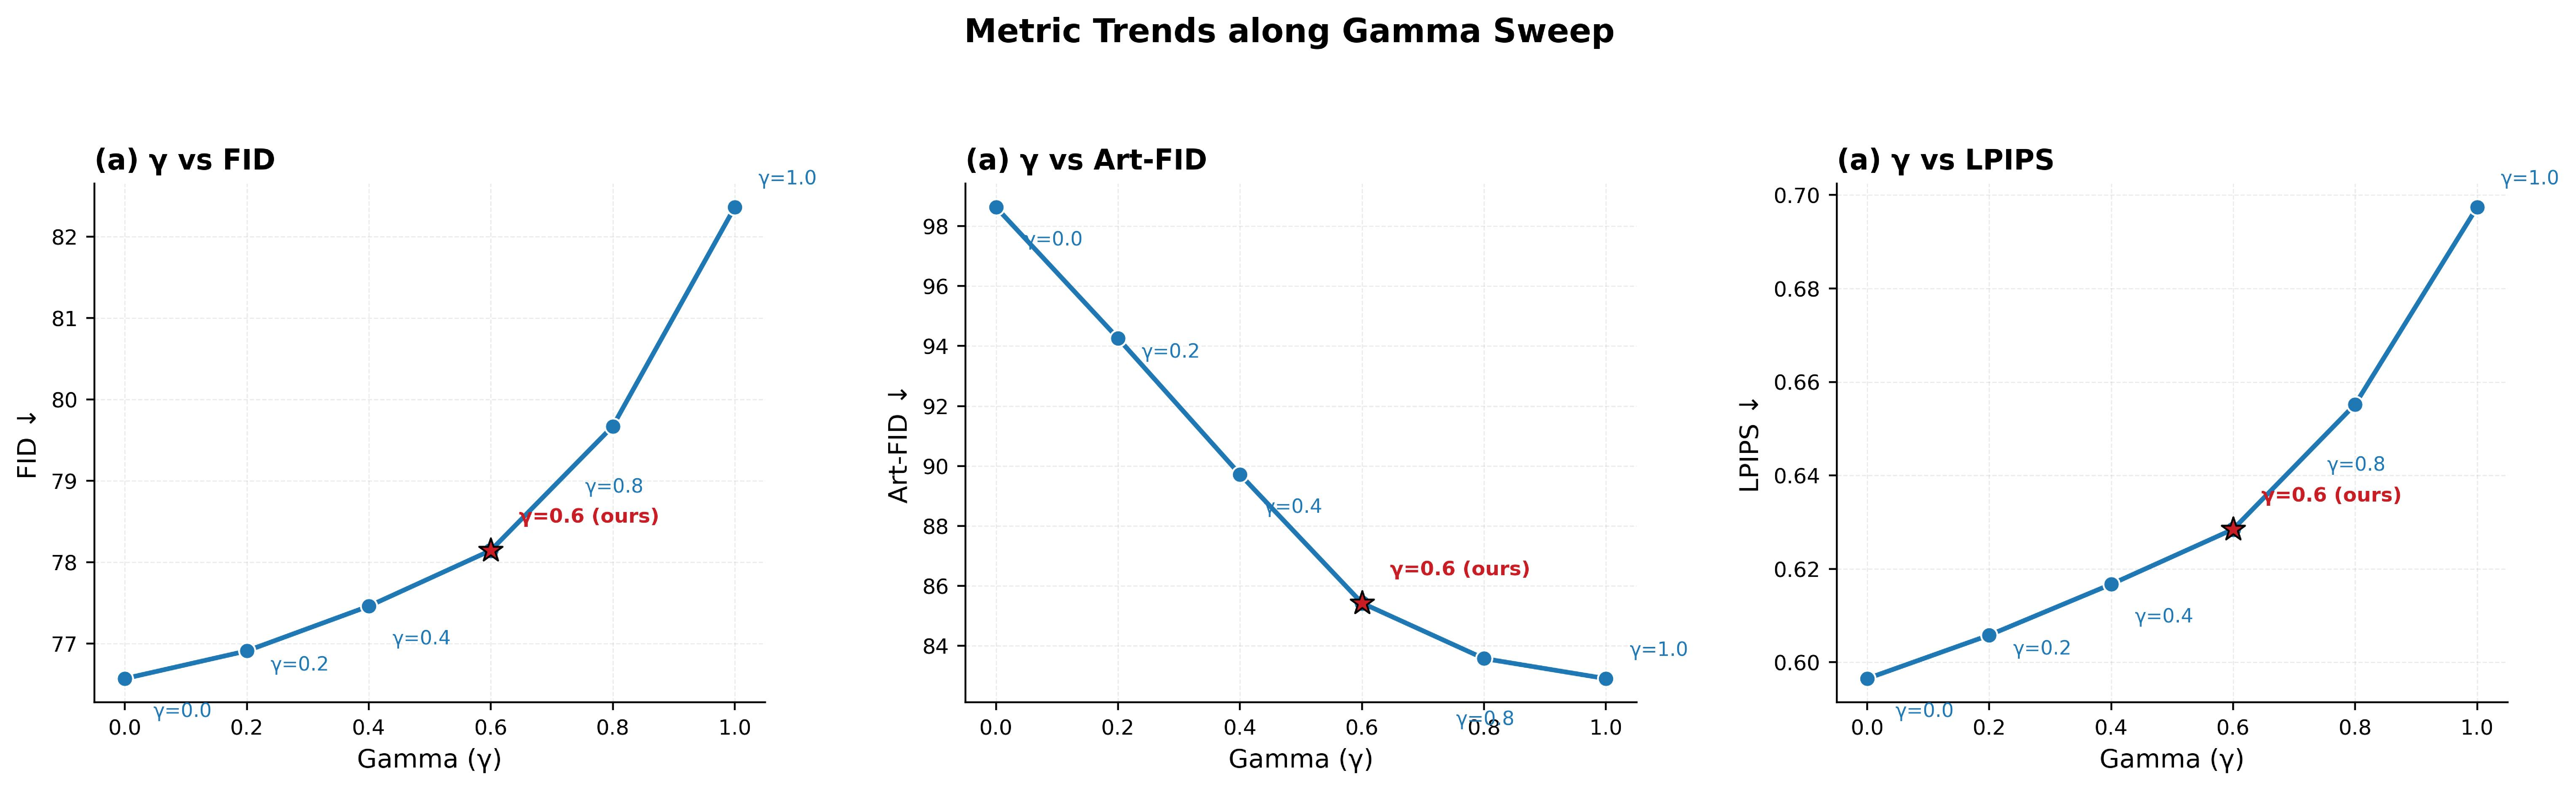
\includegraphics[width=\columnwidth]{fig_ref_comprehensive.pdf}
  \caption{Impact of $\gamma$ on FID, Art-FID, and LPIPS. As $\gamma$ increases, style fidelity generally improves but content change also increases; $\gamma=0.6$ is our adopted default trade-off point.}
  \label{fig:comprehensive}
\end{figure}

\begin{figure}[H]
  \centering
  
\includegraphics[width=\columnwidth]{fig_gamma_5blk.pdf}
  \caption{Style transfer results at different $\gamma$ values under the AdaIN-enabled 5-processor configuration in \texttt{up\_blocks.0.attentions.1} (our method). From left to right: $\gamma=0.2,0.4,0.8,1.0$, clearly illustrating the gradual enhancement of style texture as $\gamma$ increases.}
  \label{fig:gamma_5blk}
\end{figure}

\textbf{Conclusion:} As $\gamma$ gradually increases, style texture and color expression are generally enhanced, and generated results become closer to the target artistic style distribution; at the same time, content fidelity and fine-grained structure are more susceptible to degradation. Specifically, smaller $\gamma$ favors content preservation, while larger $\gamma$ favors style injection. Combining quantitative metrics with visual results in Fig.~\ref{fig:comprehensive} and Fig.~\ref{fig:gamma_5blk}, we select $\gamma=0.6$ as the default trade-off point that leans toward content stability.

\subsection{Qualitative Analysis of StyleKV Target Processor Count}

Table~\ref{tab:adain_target_blocks} has already explained that \texttt{1blk}/\texttt{2blk} belong to target block configurations in the early naive AdaIN prototype, whereas experiments prefixed with \texttt{proc} concern the number of processors within StyleKV. These are not the same ablation dimension, so this section does not compare them as a unified quantitative ablation group. To observe the impact of the number of processors within StyleKV on style injection intensity and content preservation, we fix the target block to \texttt{up\_blocks.0.attentions.1} and vary only the number of self-attention processors participating in K/V fusion within that block for qualitative visual analysis.

\begin{figure}[H]
  \centering
  
\includegraphics[width=\columnwidth]{fig_block_compare.pdf}
  \caption{Comparison of style transfer results under AdaIN-enabled 1-processor and 5-processor configurations in \texttt{up\_blocks.0.attentions.1} at different $\gamma$ values. Top row: 1-proc StyleKV configuration; bottom row: 5-proc StyleKV configuration (our method). More target processors yield stronger style injection (more pronounced style texture in the bottom row) while still maintaining good content structure in the shown examples.}
  \label{fig:block_compare}
\end{figure}

\begin{figure}[H]
  \centering
  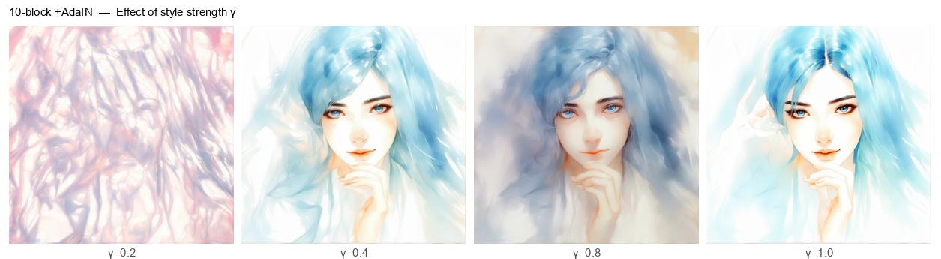
\includegraphics[width=\columnwidth]{fig_gamma_10blk.pdf}
  \caption{Style transfer results under the AdaIN-enabled 10-processor configuration in \texttt{up\_blocks.0.attentions.1} at different $\gamma$ values. Compared with the 5-proc configuration in the same block, 10-proc yields stronger style injection at the same $\gamma$, but content detail preservation is slightly inferior to the 5-proc configuration.}
  \label{fig:gamma_10blk}
\end{figure}

\textbf{Observation:} Fig.~\ref{fig:block_compare} shows that within the same target block, the 5-proc configuration yields more pronounced texture transfer compared to the 1-proc configuration, especially with more sufficient style features at higher $\gamma$ values. Fig.~\ref{fig:gamma_10blk} further indicates that the 10-proc configuration continues to enhance stylization but is more likely to degrade facial details and local structure at high $\gamma$. Considering visual quality and computational cost together, we adopt 5 processors in \texttt{up\_blocks.0.attentions.1} as the default StyleKV configuration.

\subsection{Qualitative Result Analysis}

\subsubsection{Comparison of Different Block/Processor Configurations and AdaIN Effects}

Table~\ref{tab:qual_blocks} compares the generation results of four naive AdaIN baseline configurations. Fig.~\ref{fig:adain_compare} further illustrates the impact of the AdaIN module on color coordination under the 1-block configuration.

\begin{table}[htbp]
  \centering
  \caption{Qualitative comparison of different target block counts and AdaIN configurations. Configurations using AdaIN exhibit better color coordination and more uniform style coverage; configurations without AdaIN show stronger style transfer but more noticeable content structure degradation.}
  \label{tab:qual_blocks}
  \small
  \setlength{\tabcolsep}{3pt}
  \begin{tabular}{lc>{\raggedright\arraybackslash}p{3.5cm}}
    \toprule
    Variant & \#Blocks & Observation \\
    \midrule
    adain\_1blk   & 1 & Concentrated style injection, noticeable texture transfer \\
    adain\_2blk   & 2 & Uniform style coverage, better color coordination \\
    no\_adain\_1blk & 1 & Strong style transfer, slightly inferior content preservation \\
    no\_adain\_2blk & 2 & Enhanced style injection, more blurred structure \\
    \bottomrule
  \end{tabular}
\end{table}

\begin{figure}[H]
  \centering
  
\includegraphics[width=\columnwidth]{fig_adain_compare.pdf}
  \caption{Impact of the AdaIN module on style transfer (1-block configuration). Top row: results with AdaIN; bottom row: results without AdaIN. The AdaIN module significantly improves color coordination and overall atmospheric consistency, with the difference being more pronounced at higher $\gamma$ values.}
  \label{fig:adain_compare}
\end{figure}

Fig.~\ref{fig:gallery} (the teaser at the beginning of the paper) presents the overall transfer results of our method in a comprehensive comparison.

\subsubsection{Impact of Prompts}

Prompt quality has a material effect on stylization quality. Empirically, detailed prompts that describe objects, materials, and spatial relationships yield more coherent outputs than brief, generic descriptions, consistent with the known sensitivity of text-conditioned diffusion models to prompt specificity.

\subsection{Key Experimental Findings}

\subsubsection{Trade-off Between Canny Edge Map Resolution and Inference Time}

The granularity of the Canny edge map directly affects generation quality and inference efficiency. Table~\ref{tab:resolution_canny} tests inference times at different Canny resolutions.

\begin{figure}[htbp]
  \centering
  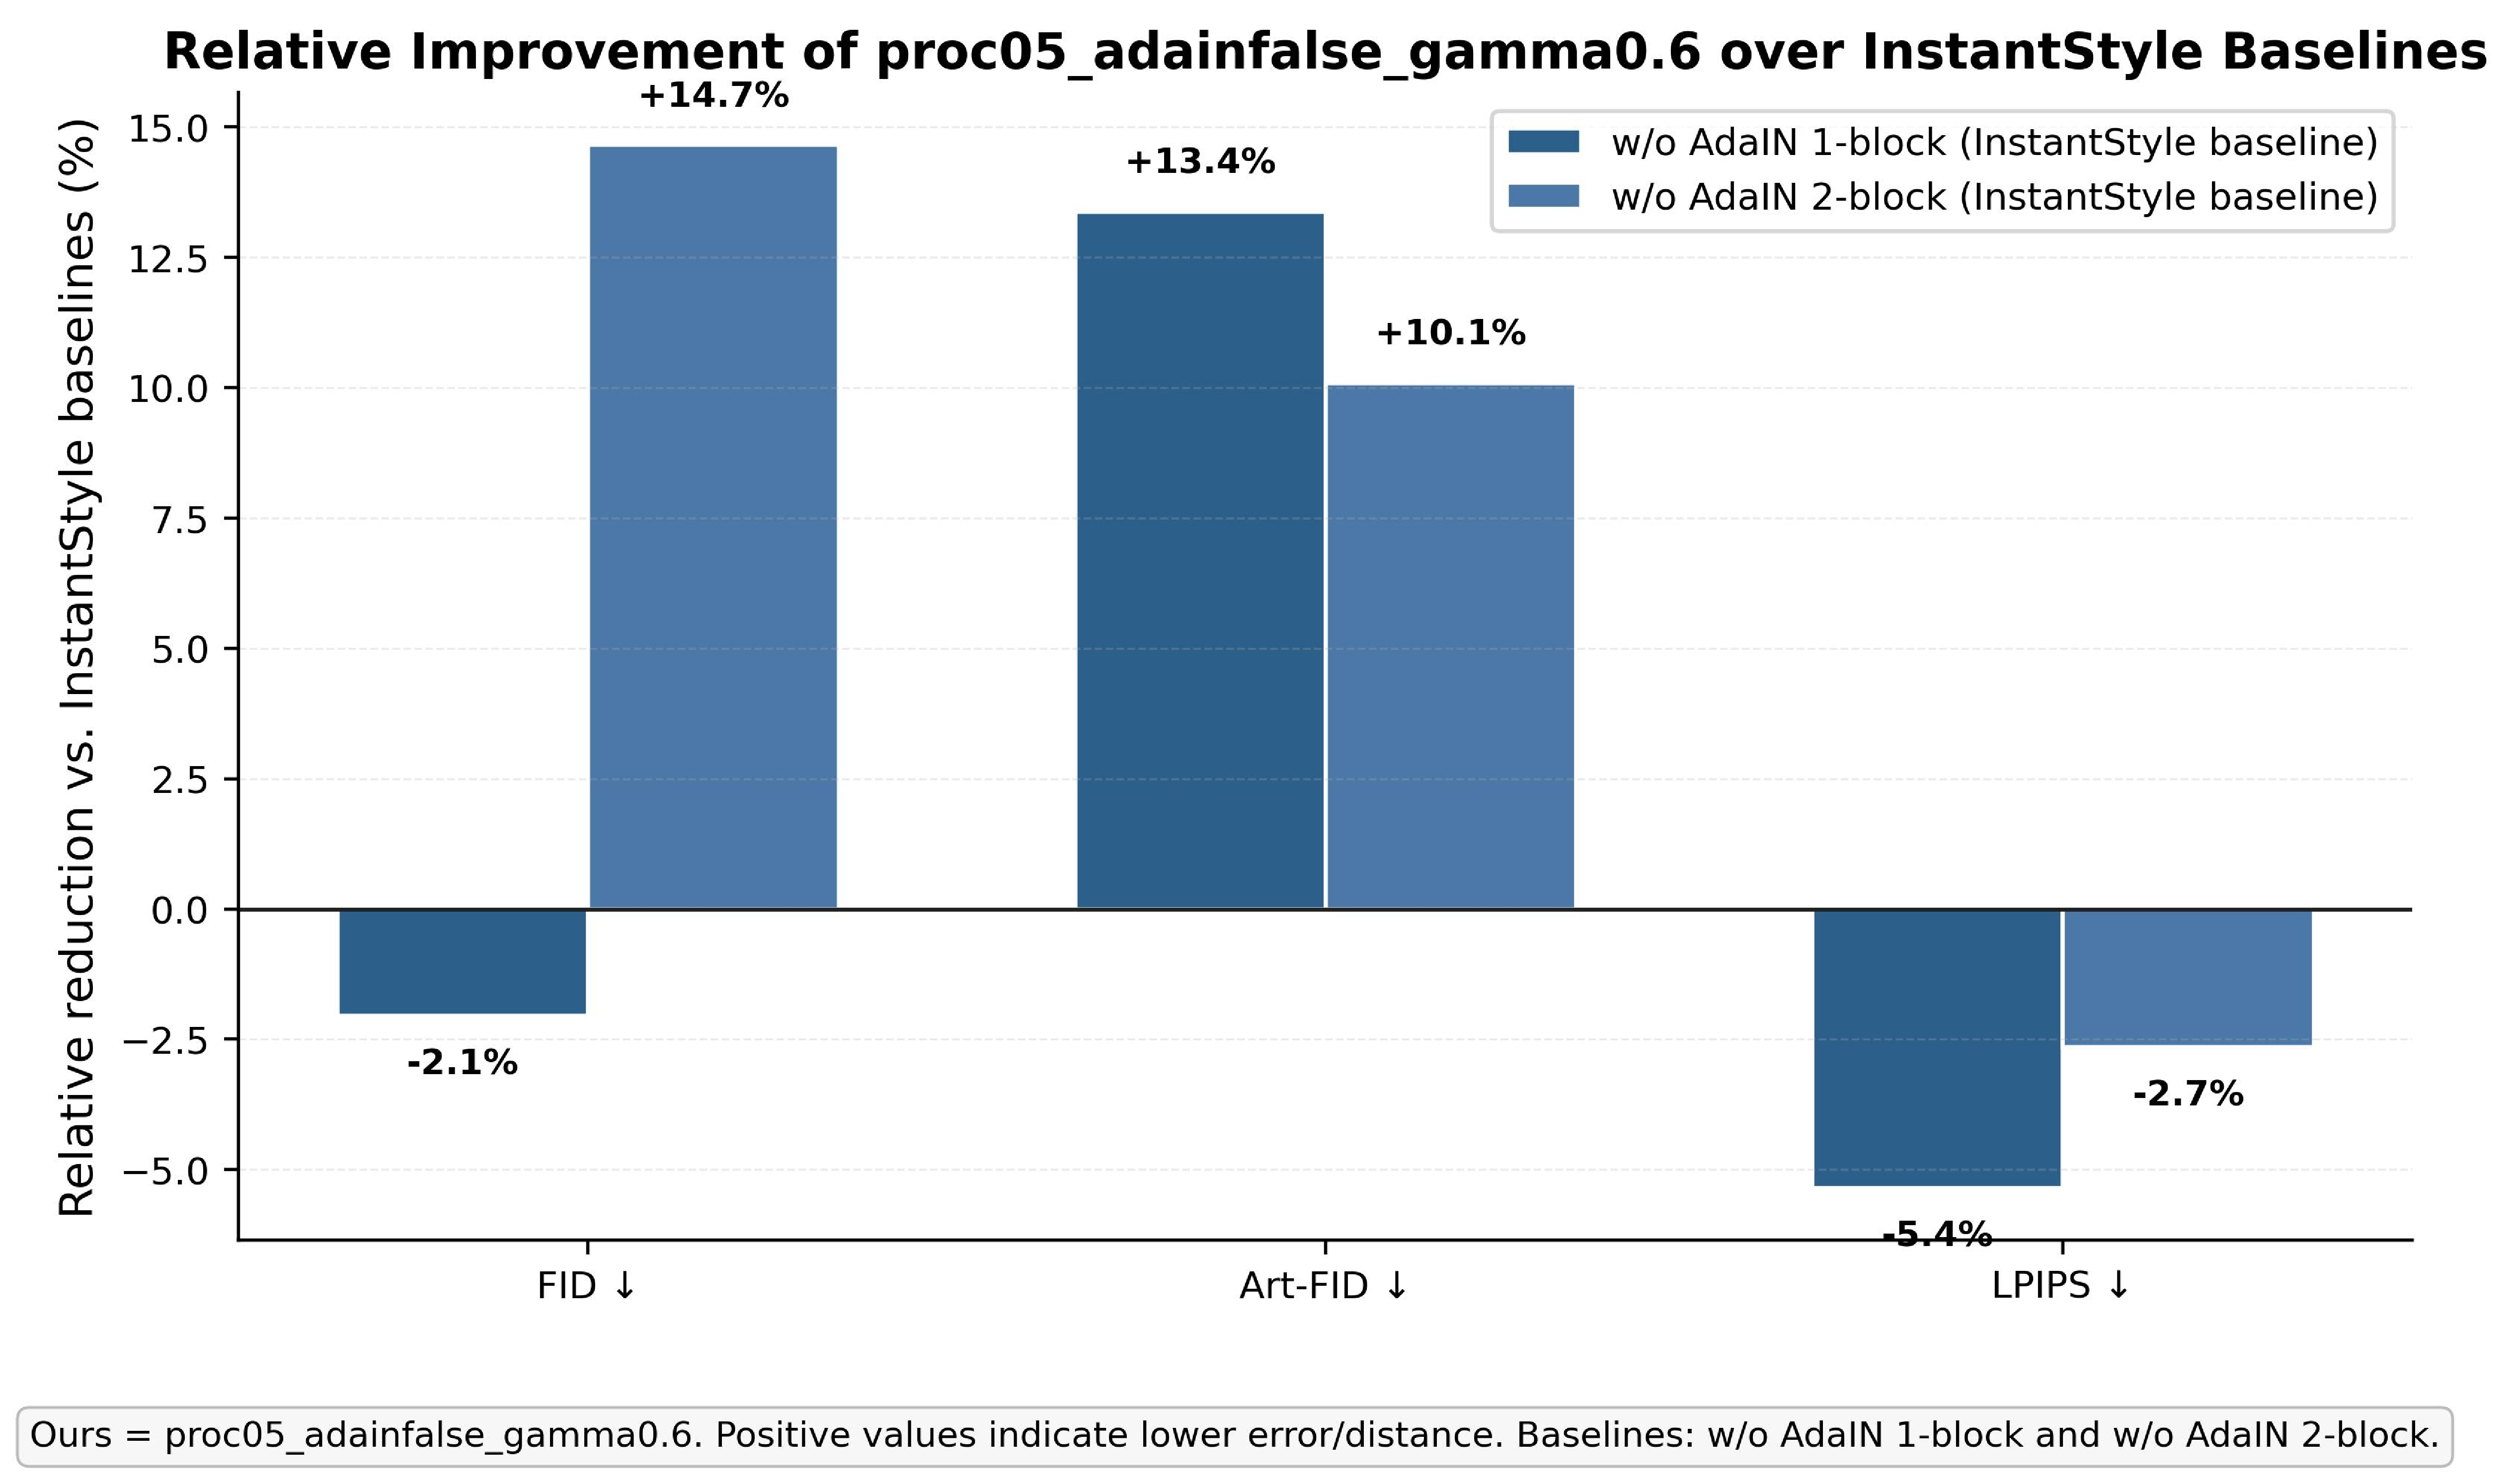
\includegraphics[width=\columnwidth]{fig_canny_res.pdf}
  \caption{Comparison of structural conditions and generation results at different Canny resolutions. Left column: Canny edge maps; right column: corresponding stylized outputs, with the reference style image embedded in the bottom-left corner of each output.}
  \label{fig:canny_res}
\end{figure}

\begin{table}[htbp]
  \centering
  \caption{Canny resolution vs.\ inference time. Higher resolution provides richer structure but increases latency and may introduce artifacts.}
  \label{tab:resolution_canny}
  \small
  \begin{tabular}{lll}
    \toprule
    Resolution & Canny Size & Time \\
    \midrule
    1080$\times$599   & same as input & $\sim$12\,s \\
    5774$\times$1536  & same as input & $\sim$68\,s \\
    \bottomrule
  \end{tabular}
\end{table}

\textbf{Key findings:} (1) Finer Canny edge maps improve generation quality, as the model receives richer structural information; (2) however, excessively fine edge maps may cause the model to over-respond to local edges, producing outlining artifacts, fragmented textures, or unnatural local details; (3) inference time increases markedly with Canny resolution; (4) a balance must be struck between too fine (many artifacts, high cost) and too coarse (loss of detail). As shown in Fig.~\ref{fig:canny_res}, the difference in Canny edge detection granularity across resolutions is significant. Based on these observations, the frontend supports dynamic adjustment of Canny edge detection parameters by the user.

\subsubsection{Device Resource Constraints}

Diffusion models (Stable Diffusion base model $\sim$7--8\,GB, plus VAE, ControlNet, and feature caching modules, totaling $\sim$15--20\,GB of VRAM) still pose certain challenges for consumer-grade GPUs. Even with a V100-32\,GB, batch generation faces VRAM pressure and GPU resource contention. Compared with performing injection across more blocks or processors, our approach adopts selective processor injection within \texttt{up\_blocks.0.attentions.1} (5 self-attention processors by default), thereby controlling the additional computation and caching overhead so that the entire pipeline can run smoothly on a V100.

%% ================================================
%% 5. Interactive Frontend
%% ================================================
\section{Interactive Frontend}

To enhance practical usability and user experience, we built an interactive frontend called \textbf{StyleKV Control Studio} based on the Gradio framework.

\subsection{Frontend Functional Modules}

{\bfseries (1) Image Input Module:} content image upload, style image upload, automatic generation and preview of the Canny edge map.

{\bfseries (2) Prompt Control Module:} positive prompt (describing the desired generation result), negative prompt (elements to avoid), with support for long text input.

{\bfseries (3) ControlNet/Canny Parameter Adjustment:} Canny Low/High Threshold (edge detection sensitivity), Conditioning Scale (ControlNet control strength), Bilateral Filter parameters (edge preprocessing denoising).

{\bfseries (4) AdaIN Style Fusion Module:} AdaIN Alpha (fusion intensity), AdaIN Beta (fusion bias), with real-time preview support.

{\bfseries (5) Generation Parameter Control:} Steps (DDIM sampling steps), CFG Scale (classifier-free guidance), Seed (random seed), KV fusion intensity $\gamma$.

{\bfseries (6) Output Management:} output directory setting, real-time generation status display, result gallery showcase.

\subsection{Frontend Features and Value}

The frontend supports hot parameter reloading (adjusting parameters without restarting to view results), real-time Canny edge map preview, saving configurations as JSON files, and batch generation. The design goal is to lower the usage barrier, enabling non-expert users to understand the impact of each parameter on generation results through intuitive sliders, switches, and preview images. Fig.~\ref{fig:gradio} shows the overall interface layout of the frontend.

\begin{figure}[htbp]
  \centering
  
\includegraphics[width=\columnwidth]{fig_gradio.pdf}
  \caption{Interface of the StyleKV Control Studio interactive frontend. Through the left panel, users can upload content and style images, adjust ControlNet/Canny parameters, set AdaIN fusion coefficients, and configure generation parameters; the right panel displays real-time Canny edge map previews and stylized output results.}
  \label{fig:gradio}
\end{figure}

%% ================================================
%% 6. Future Work
%% ================================================
\section{Future Work}

\subsection{Quantitative Comparison with Existing Methods}
The experiments in this paper are limited to self-ablation; head-to-head comparison with InST [12], StyleDiffusion [13], and InstantStyle [17] under a unified protocol remains necessary to contextualize the reported gains.

\subsection{Adaptive Canny Edge Map Generation}
Canny thresholds are currently set manually. Integrating learned edge extractors such as HED or RINDNet could yield adaptive edge maps that reduce per-image tuning without sacrificing structural fidelity.

\subsection{VLM-Based Automatic Prompt Generation}
Prompt writing remains a manual bottleneck. Open-source vision-language models (e.g., Qwen-VLM, LLaVA) could be integrated to generate high-quality style-aware prompts automatically.

\subsection{Cross-Architecture Adaptation and Lightweighting}
The effective-processor selection strategy is tied to the SDXL architecture. Extending the KV fusion mechanism to SD1.5, SD3, and other backbones would require re-identifying salient attention processors per architecture. Distillation and quantization could further reduce the VRAM footprint for consumer-grade deployment.

\subsection{Incorporating Tile ControlNet}
High-resolution Canny edge maps risk introducing outlining artifacts. Tile ControlNet offers a patch-wise processing strategy that could mitigate these artifacts while preserving fine detail.

\subsection{Processor-Level Contribution Analysis}
A systematic, per-processor ablation across the full UNet would clarify which self-attention processors drive different style attributes, providing a principled basis for injection-site selection beyond the current empirical configuration.

\subsection{Multi-Condition ControlNet Fusion}
Only Canny edges are used at present. Combining multiple ControlNet conditions (edge, depth, pose) could reinforce content structure along complementary spatial dimensions.

%% ================================================
%% 7. Conclusion and Limitations
%% ================================================
\FloatBarrier
\section{Conclusion and Limitations}

\subsection{Conclusion}

This paper presented AdaIN StyleKV, a training-free style transfer framework operating on a frozen SDXL+ControlNet backbone. The method combines three mechanisms: selective KV fusion within a subset of self-attention processors in \texttt{up\_blocks.0.attentions.1}, controlled by a scalar $\gamma$; cross-modal AdaIN adapted from StyleStudio [31] to align text-condition features with style-image color statistics; and Canny ControlNet for spatial structure preservation. On 5000 COCO$\times$WikiArt pairs, the full configuration achieves Art-FID 90.76 with LPIPS 0.599, while the AdaIN-free StyleKV variant reaches Art-FID 85.43 at the cost of higher perceptual disruption (LPIPS 0.629). An accompanying Gradio interface, StyleKV Control Studio, provides real-time control over all parameters. Key empirical findings from this study include the sensitivity of stylization quality to Canny edge-map resolution, the impact of prompt specificity on output coherence, and the observation that AdaIN systematically trades style-domain alignment for perceptual stability---a trade-off that future work should characterize more precisely across diverse style categories and model architectures.

\subsection{Limitations}

Although our method achieves favorable results, the following limitations remain, as listed in Table~\ref{tab:limitations}. These limitations also constitute the key focus areas of the future work outlined in Section~6.

\begin{table}[htbp]
  \centering
  \caption{Major limitations of our method and corresponding improvement directions.}
  \label{tab:limitations}
  \small
  \setlength{\tabcolsep}{3pt}
  \begin{tabular}{>{\raggedright\arraybackslash}p{2.0cm}>{\raggedright\arraybackslash}p{3.0cm}>{\raggedright\arraybackslash}p{2.6cm}}
    \toprule
    Limitation & Description & Improvement \\
    \midrule
    No external SOTA comparison & Only self-variant ablation; not compared with InST, StyleDiffusion, InstantStyle, etc. & Reproduce and compare under unified protocol \\
    Insufficient processor ablation & Only tested few processor configs in \texttt{up0.attn1} & Full processor-level contribution analysis \\
    Single ControlNet & Only Canny tested; other modalities not explored & Multi-condition ControlNet fusion \\
    External prompt dependency & Prompts from external models; no integrated VLM & Integrate Qwen-VLM / LLaVA \\
    Limited evaluation metrics & FID, Art-FID, LPIPS only; no perceptual/semantic coverage & Add metrics + human subjective study \\
    High device requirements & Needs V100-class GPU; not consumer-friendly & Distillation \& quantization \\
    \bottomrule
  \end{tabular}
\end{table}

\subsection{Future Outlook}

Style transfer remains an open problem, and several directions merit further investigation. Training-free methods would benefit from finer-grained style disentanglement, enabling independent control over brush scale, palette, and texture density. Multi-condition fusion---combining text, reference images, and color palettes without destructive interference---deserves systematic study. A rigorous characterization of which UNet layers contribute to style transfer would enable more parameter-efficient architectures. Finally, distillation and quantization could bring these pipelines to consumer hardware, substantially expanding their practical deployability.

%% ================================================
%% Acknowledgments
%% ================================================
\section*{Acknowledgments}
We are grateful to the AutoDL platform for GPU resources and to the open-source community behind Stable Diffusion, ControlNet, and the diffusers library---without these foundations this project wouldn't have been possible.

%% ================================================
%% References
%% ================================================
\begin{thebibliography}{99}

\bibitem{efros1999} A.~A.~Efros and T.~K.~Leung, ``Texture synthesis by non-parametric sampling,'' in \emph{Proc. ICCV}, 1999.

\bibitem{gatys2016} L.~A.~Gatys, A.~S.~Ecker, and M.~Bethge, ``Image style transfer using convolutional neural networks,'' in \emph{Proc. CVPR}, 2016.

\bibitem{ulyanov2016} D.~Ulyanov, V.~Lebedev, A.~Vedaldi, and V.~Lempitsky, ``Texture networks: Feed-forward synthesis of textures and stylized images,'' in \emph{Proc. ICML}, 2016.

\bibitem{huang2017} X.~Huang and S.~Belongie, ``Arbitrary style transfer in real-time with adaptive instance normalization,'' in \emph{Proc. ICCV}, 2017.

\bibitem{zhu2017} J.-Y.~Zhu, T.~Park, P.~Isola, and A.~A.~Efros, ``Unpaired image-to-image translation using cycle-consistent adversarial networks,'' in \emph{Proc. ICCV}, 2017.

\bibitem{choi2018} Y.~Choi, M.~Choi, M.~Kim, J.-W.~Ha, S.~Kim, and J.~Choo, ``StarGAN: Unified generative adversarial networks for multi-domain image-to-image translation,'' in \emph{Proc. CVPR}, 2018.

\bibitem{karras2019} T.~Karras, S.~Laine, and T.~Aila, ``A style-based generator architecture for generative adversarial networks,'' in \emph{Proc. CVPR}, 2019.

\bibitem{sohl2015} J.~Sohl-Dickstein, E.~A.~Weiss, N.~Maheswaranathan, and S.~Ganguli, ``Deep unsupervised learning using nonequilibrium thermodynamics,'' in \emph{Proc. ICML}, 2015.

\bibitem{ho2020} J.~Ho, A.~Jain, and P.~Abbeel, ``Denoising diffusion probabilistic models,'' in \emph{Proc. NeurIPS}, 2020.

\bibitem{song2020} Y.~Song and S.~Ermon, ``Improved techniques for training score-based generative models,'' in \emph{Proc. NeurIPS}, 2020.

\bibitem{rombach2022} R.~Rombach, A.~Blattmann, D.~Lorenz, P.~Esser, and B.~Ommer, ``High-resolution image synthesis with latent diffusion models,'' in \emph{Proc. CVPR}, 2022.

\bibitem{zhang2023inst} Y.~Zhang, N.~Huang, F.~Tang, H.~Huang, C.~Ma, W.~Dong, and C.~Xu, ``InST: Inversion-based style transfer with diffusion models,'' in \emph{Proc. CVPR}, 2023.

\bibitem{wang2023style} Z.~Wang, L.~Zhao, W.~Xing, and D.~Lu, ``StyleDiffusion: Controllable disentangled style transfer via diffusion models,'' in \emph{Proc. ICCV}, 2023.

\bibitem{jeong2023} J.~Jeong, M.~Kwon, and Y.~Uh, ``DiffStyle: Training-free style transfer with diffusion models,'' \emph{arXiv preprint arXiv:2312.01714}, 2023.

\bibitem{zhang2023controlnet} L.~Zhang, A.~Rao, and M.~Agrawala, ``Adding conditional control to text-to-image diffusion models,'' in \emph{Proc. ICCV}, 2023.

\bibitem{hertz2023} A.~Hertz, R.~Mokady, J.~Tenenbaum, K.~Aberman, Y.~Pritch, and D.~Cohen-Or, ``Style Injection: Training-free style transfer using self-attention,'' \emph{arXiv preprint arXiv:2312.08008}, 2023.

\bibitem{wang2024instantstyle} H.~Wang, Q.~Wang, X.~Bai, Z.~Qin, and A.~Chen, ``InstantStyle: Free lunch towards style-preserving in text-to-image generation,'' \emph{arXiv preprint arXiv:2404.02733}, 2024.

\bibitem{lin2014} T.-Y.~Lin, M.~Maire, S.~Belongie, J.~Hays, P.~Perona, D.~Ramanan, P.~Doll\'{a}r, and C.~L.~Zitnick, ``Microsoft COCO: Common objects in context,'' in \emph{Proc. ECCV}, 2014.

\bibitem{wikiart} WikiArt, ``WikiArt Visual Art Encyclopedia.'' [Online]. Available: \url{https://www.wikiart.org/}.

\bibitem{artfid} M.~Wright and B.~Ommer, ``ArtFID: Quantitative evaluation of neural style transfer,'' in \emph{Proc. GCPR}, 2022, arXiv:2207.12280.

\bibitem{heusel2017} M.~Heusel, H.~Ramsauer, T.~Unterthiner, B.~Nessler, and S.~Hochreiter, ``GANs trained by a two time-scale update rule converge to a local Nash equilibrium,'' in \emph{Proc. NeurIPS}, 2017.

\bibitem{zhang2018lpips} R.~Zhang, P.~Isola, A.~A.~Efros, E.~Shechtman, and O.~Wang, ``The unreasonable effectiveness of deep features as a perceptual metric,'' in \emph{Proc. CVPR}, 2018.

\bibitem{simonyan2015} K.~Simonyan and A.~Zisserman, ``Very deep convolutional networks for large-scale image recognition,'' in \emph{Proc. ICLR}, 2015.

\bibitem{johnson2016} J.~Johnson, A.~Alahi, and L.~Fei-Fei, ``Perceptual losses for real-time style transfer and super-resolution,'' in \emph{Proc. ECCV}, 2016.

\bibitem{liu2021} S.~Liu, T.~Lin, D.~He, F.~Li, M.~Wang, X.~Li, Z.~Sun, Q.~Li, and E.~Ding, ``AdaAttN: Revisit attention mechanism in arbitrary neural style transfer,'' in \emph{Proc. ICCV}, 2021.

\bibitem{deng2022} Y.~Deng, F.~Tang, W.~Dong, C.~Ma, X.~Pan, L.~Wang, and C.~Xu, ``StyTr$^2$: Image style transfer with transformers,'' in \emph{Proc. CVPR}, 2022.

\bibitem{an2021} J.~An, S.~Huang, Y.~Song, D.~Dou, W.~Liu, and J.~Luo, ``ArtFlow: Unbiased image style transfer via reversible neural flows,'' in \emph{Proc. CVPR}, 2021.

\bibitem{chen2021dualast} H.~Chen, L.~Zhao, Z.~Wang, H.~Zhang, Z.~Zuo, A.~Li, W.~Xing, and D.~Lu, ``DualAST: Dual style-learning networks for artistic style transfer,'' in \emph{Proc. CVPR}, 2021.

\bibitem{karras2020} T.~Karras, S.~Laine, M.~Aittala, J.~Hellsten, J.~Lehtinen, and T.~Aila, ``Analyzing and improving the image quality of StyleGAN,'' in \emph{Proc. CVPR}, 2020.

\bibitem{karras2021} T.~Karras, M.~Aittala, S.~Laine, E.~H\"{a}rk\"{o}nen, J.~Hellsten, J.~Lehtinen, and T.~Aila, ``Alias-free generative adversarial networks,'' in \emph{Proc. NeurIPS}, 2021.

\bibitem{lei2025stylestudio} M.~Lei, X.~Song, B.~Zhu, H.~Wang, and C.~Zhang, ``StyleStudio: Text-driven style transfer with selective control of style elements,'' in \emph{Proc. CVPR}, 2025.

\end{thebibliography}

%% ================================================
%% Appendix
%% ================================================
\FloatBarrier
\section*{Appendix}
\begingroup
\titlespacing*{\subsection}{0pt}{0.45em}{0.2em}

\subsection*{A. Complete Data of the 7 Variants}

Table~\ref{tab:appendix_a} lists the complete experimental data of the 7 variants, consistent with Table~\ref{tab:quant_results} in the main text.

\begin{center}
  \centering
  \small
  \captionof{table}{Complete quantitative data of the 7 variants (consistent with Table~5 in the main text).}
  \label{tab:appendix_a}
  \vspace{-2pt}
  \begin{tabular}{lccc}
    \toprule
    Variant Name & FID$\downarrow$ & Art-FID$\downarrow$ & LPIPS$\downarrow$ \\
    \midrule
    V1 (adain\_1blk)       & 73.34 & 103.17 & 0.581 \\
    V2 (adain\_2blk)       & 88.54 & 98.42  & 0.599 \\
    V3 (no\_adain\_1blk)   & 76.57 & 98.63  & 0.597 \\
    V4 (no\_adain\_2blk)   & 91.56 & 95.02  & 0.612 \\
    V5 (adain\_no\_ctrl)   & 70.75 & 104.12 & 0.746 \\
    V6 (proc05\_no\_adain) & 78.14 & 85.43  & 0.629 \\
    V7 (proc05\_adain)     & 78.48 & 90.76  & 0.599 \\
    \bottomrule
  \end{tabular}
\end{center}

\subsection*{B. Complete Gamma Ablation Experiment Data}

Table~\ref{tab:appendix_b} lists the complete data of the $\gamma$ experiment, consistent with Table~\ref{tab:gamma_ablation} in the main text.

\begin{center}
  \centering
  \small
  \captionof{table}{Complete $\gamma$ ablation experiment data (5-processor configuration in \texttt{up\_blocks.0.attentions.1} + AdaIN + ControlNet, consistent with Table~6 in the main text).}
  \label{tab:appendix_b}
  \vspace{-2pt}
  \begin{tabular}{cccc}
    \toprule
    $\gamma$ & FID$\downarrow$ & Art-FID$\downarrow$ & LPIPS$\downarrow$ \\
    \midrule
    0.0 & 76.57 & 98.63 & 0.597 \\
    0.2 & 76.91 & 94.26 & 0.606 \\
    0.4 & 77.46 & 89.72 & 0.617 \\
    0.6 & 78.48 & 90.76 & 0.599 \\
    0.8 & 79.67 & 83.58 & 0.655 \\
    1.0 & 82.36 & 82.91 & 0.697 \\
    \bottomrule
  \end{tabular}
\end{center}

\endgroup

\end{document}
